Plaçons nous dans le contexte physique naturel des équations d'advection, diffusion, réaction:
Des particules sont placées dans un milieu fluide où elles \textbf{diffusent}, ce milieu fluide
est en mouvement, cet écoulement déplace les particules, il les \textbf{advecte}.
Enfin les particules \textbf{réagissent} entre-elles et ces réactions modifient les grandeurs thermodynamiques (température, pression) et \textit{in fine} les propriétés
du milieu fluide.
Les équations d'advection, diffusion, réaction modélisent donc ces trois phénomènes et leurs couplages respectifs.

\subsection{Les trois opérateurs}
\subsubsection{Advection}
    L'advection désigne le transport d'une quantité par un flot. L'opérateur d'advection le plus simple est l'opérateur
    de transport $c \frac{\partial}{\partial x}$:
    \begin{align}\frac{\partial u}{\partial t} = c \frac{\partial u}{\partial x}\end{align}
    De manière générale un opérateur d’advection d'une quantité $u$ par un flot $\underline a$ s'écrit $\underline a \cdot \underline{\nabla} u$.
    Par exemple dans les équations de Navier-Stokes, l'opérateur $\underline{v} \cdot \underline{\underline \nabla} \, \underline{v}$ représente 
    la vitesse $\underline v$ qui est transportée par elle même. Une version simplifiée de ce phénomène est l'équation bien connue de Bürgers.\par 
    Les opérateurs d'advections sont généralement à valeurs propres imaginaires\footnote{Par abus, s'il s'agit d'un opérateur non-linéaire on lui associera les valeurs propres de sa Jacobienne.}.
    Ainsi ils sont peu raides mais résonnants. Les méthodes explicites sont généralement les plus adaptées pour les traiter.
    %       AFAIRE ---> trouver une référence pour justifier que les opérateurs d'advections sont à valeurs propres imaginaires.

\subsubsection{Diffusion}
    La diffusion désigne l'\textit{éparpillement} de particules au sein d'un milieu fluide
    \footnote{En théorie de l'information cela décrit la tendance de l'entropie augmenter et l'information à se moyenner, se flouter.}.
    Ce phénomène est la limite macroscopique du déplacement microscopiques 
    des particules à cause de l'agitation thermique. L'opérateur de diffusion le plus classique est celui de l'équation de la chaleur:
    \begin{align} \frac{\partial u}{\partial t} = D \Delta u.\end{align}
    Le spectre de cet opérateur est $\mathbb R^-$, il est donc infiniment raide. Lorsqu'il est discrétisé seul une partie de sa raideur est captée,
    en pratique la raideur de l'opérateur augmente de manière quadratique avec la finesse de la discrétisation spatiale.\par
    %       AFAIRE ---> trouver une référence (ou faire la démo) pour le spectre.
    Cet opérateur est donc moyennement raide. Ainsi on pourrait penser qu'une méthode implicite est adéquate. Cependant ce n'est généralement pas le cas.
    En effet le coefficient de diffusion est généralement fonction de la température, et donc l’opérateur $D(T) \times \Delta(\cdot)$ varie génialement dans le temps et l'espace. 
    Ainsi il faut inverser à chaque itération l'opérateur implicite, et comme c'est un opérateur non local
    \footnote{Si l'opérateur de diffusion était local on pourrait résoudre plusieurs petit systèmes, potentiellement en parallèle ce qui est bien moins coûteux qu'inverser 
    un grand système. Pour se convaincre, inverser un matrice pleine de taille $10^6$ coûte au moins $10^{18}$ opérations, alors qu'inverser 100 systèmes de taille $10^4$
    coûte $100 \times 10^{12} = 10^{14}$ soit dix mille fois moins, et si ces résolution étaient parallélisé ce serait un million de fois moins.},
    il faut inverser une matrice de taille $d >> 1$ dont la structure
    peut être très hétérogène.
    (car le coefficient de diffusion dépend de $T$ et du milieu, donc \textit{in fine} de $\underline x$). Aujourd'hui il est d'usage d'utiliser 
    des méthodes explicites stabilisées qui parviennent à gérer la raideur moyenne\footnote{Nous reviendrons sur ce qualificatif au prochain paragraphe.} comme les méthodes 
    ROK2 et ROK4\cite{abdulle2002fourth}.

\subsubsection{Réaction}
    Les phénomène sont en général bien adaptés aux méthodes implicites car extrêmement raides et locaux.
    En effet,les temps typiques d'une réaction chimique\footnote{
    En réalité une réaction chimique simple (une simple combustion $H_2/O_2$ fait intervenir une dizaine de composés et reactions intermédiaires, dont les temps typiques sont très faibles.)} sont de l'ordre de la nano-seconde.
    %AFAIRE AJOUTER UNE JUSTIFICATION
    De fait, les réactions chimiques sont très difficiles à simuler par des méthodes explicites.
    Et les méthodes implicites ne sont pas très chères dans ce contexte, en effet comme les réactions sont locales 
    (à chaque pas de temps les particules les particules au sein d'une cellules ne réagissent qu'avec les autres particules de la même cellule)
    les méthodes explicites peuvent se paralléliser. En d'autres termes il est possible de mettre en oeuvre une méthode implicite par cellule,
    ce qui revient à inverser un opérateur de petite dimension en chaque cellule, et il n'est pas nécessaire d'inverser un énorme système.

\subsection{Difficultés mathématiques intrinsèques}
    La simulations des équations d'advections-réaction-diffusion se heurte à deux difficultés majeur, le couplage des trois opérateurs mentionnés précédemment
    et le caractère multi-échelles des solutions.

    \subsubsection{Première difficulté: le couplage des opérateurs}
        Les développements précédents auront convaincu le lecteur que résoudre chaque phénomène individuellement, n'est pas insurmontable. 
        Cependant, les résoudre tous en même temps, c'est à dire les coupler, est en pratique très difficile.
        En effet, lorsque l'on couple les trois opérateurs, il en résulte un unique opérateur qui doit être traité par une méthode numérique.
        C'est là que surgissent les difficultés: si la méthode est explicite (éventuellement stabilisée), la raideur de la réaction impose des pas de temps extrêmement restrictifs,
        à l'inverse si l'on choisit une méthode implicite, la non-localité de la diffusion demande l'inversion d'un système de taille déraisonnable. 
        Cette approche naïve, monolithique, n'est donc pas adaptée. Il faut trouver d'autres stratégies de pour simuler ces équations d’advection-réaction-diffusion.

    \subsubsection{Seconde difficulté: le caractère multi-échelles des solutions}
        Les solutions des solutions étudiées sont souvent multi-échelles, en temps et en espace. Cela signifie que certaines zones spatio-temporelles nécessitent
        une finesse d'approximation élevée pour pouvoir reproduire fidèlement le comportement physique, alors qu'en d'autres zones une approximation
        grossière est suffisante. Prenons l'exemple d'un incendie dans un local. Au début le foyer est très restreint et seul cette zone doit être maillée finement, 
        car partout ailleurs \textit{il ne se passe rien}, petit à petit l'incendie se propage et la zone à mailler finement augmente. Un autre exemple de phénomène 
        multi-échelle serait une détonation, il faut mailler finement, au foyer de l'explosion et le front de l'onde de choc. Mais la zone non atteinte par l'explosion, 
        qui n'a pas encore reçu le choc, pourrait être maillée très grossièrement. 
        Ainsi si l'on maille naïvement, il est envisageable qu'à certains instants, 90\% du domaine soit maillé avec un pas d'espace 100 fois plus fin que nécessaire;
        il y a alors une grande inefficacité\footnote{À cela s'ajoute le fait que ce problème augmente fortement avec la dimension.}.


\subsection{Les stratégies de simulation}
    Pour surmonter ces difficultés, des stratégies d'adaptation de maillage et d'intégration en temps spécifiques doivent être utilisées de concert. 
    \subsubsection{L'adaptation de maillage}
    Pour prendre avantage du caractère multi-échelle des solutions étudiées, il est courant de procéder à de l'adaptation de maillage.
    C'est à dire mailler avec une finesse différentes chaque zone du domaine et être en mesure de faire évoluer ce maillage de concorde avec l'évolution du problème dans le temps.
    La méthode d'adaption de maillage sur lequel nous nous concentrons est la multirésolution-adaptative par transformée d'ondelettes introduite par Ami Harten dans les années 1990 \cite{harten1994}.
    Cette méthode est très étudiée par l'équipe du CMAP et a donnée lieu au développement du logiciel Samurai\footnote{\href{https://github.com/hpc-maths/samurai}{https://github.com/hpc-maths/samurai}}.
    \begin{figure}[h]
    \centering
    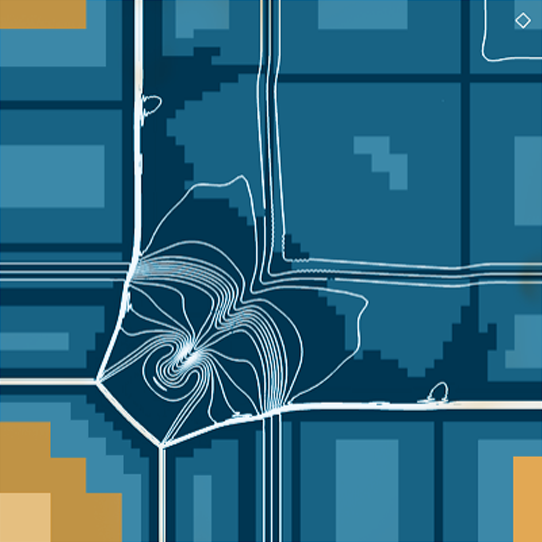
\includegraphics[width=0.5\textwidth]{media/3_/3_/exemple_compression_samurai.png}
    \caption{Exemple de maillage adapté par multiresoltion adaptative grâce au logiciel \href{https://github.com/hpc-maths/samurai}{Samurai}.}
    \label{fig:samurai}
    \end{figure}

        \paragraph{La multi-résolution adaptative}
        La multiresoltion adaptative se base sur une compression de la solution par transformée d'ondelette\footnote{C'est même procédé qui est à l'oeuvre dans la compression d'image \texttt{jpg}.}.
        Les détails mathématiques seront données plus tard et s’appuieront notamment sur \cite{postePoly}. Pour l'heure le lecteur doit simplement comprendre que la compression se fait de la manière suivante:
        une transformée en ondelette permet de représenter la solution sur différentes échelle d'espace\footnote{Par exemple les échelles $\Delta x, \Delta x/2,\Delta x/4,\dots, \Delta x/2^n$}. 
        Cela permet de quantifier l'information contenue à en chaque échelle d'espace. Enfin la compression consiste à ignorer les échelles ne comprenant pas assez d'information
        par rapport à un seuil $\varepsilon$ fixé par l'utilisateur.

        \paragraph{Autres méthodes}
        Il existe d'autre stratégies pour raffiner le maillage autour des zones sensibles que la transformée en ondelette. 
        La plus classique est une adaptation basée sur les gradients. Si les gradients sont élevés c'est que la solution est complexe,
        et donc un maillage fin est nécessaire pour la représenter fidèlement. Cette approche est simple à mettre en oeuvre et part de la même heuristique 
        que la multiresoltion adaptative, cependant elle est moins systématique (pas de quantification de l'information perdue) et plus difficile à analyser. 
        Elle est cependant utilisée dans des logiciels industriels comme Ansys 
        \footnote{\href{https://w.ww.ansys.com/fr-fr/blog/how-to-accelerate-ansys-fluent-simulations-with-adaptive-meshing}{https://www.ansys.com/fr-fr/blog/how-to-accelerate-ansys-fluent-simulations-with-adaptive-meshing}}.
        % AFAIRE : ajouter une ref pour les adaptations basées sur les gradients, une justification sur le caractère moins facile a analyser et éventuellement d'autres méthodes de raffinement.

    \subsubsection{Les techniques d'intégration}
        Comme expliqué précédemment, la simulation de chaque opérateur est faisable individuellement mais très difficile conjointement.
        Les stratégies pour intégrer les trois opérateurs en même temps, reposent donc sur le fait de les intégrer... séparément.

        \paragraph{La séparation d'opérateurs}
            La séparation d'opérateurs (en Anglais: \textit{splitting}) consiste à intégrer successivement chaque opérateur.
            L'intégration d'un opérateur $A$, dans une équation comme :
            \begin{align}\frac{\partial u}{\partial t} = Au.\end{align}
            s'écrit avec la notion d'exponentielle de matrice\footnote{Ou de manière plus rigoureuse avec la notion de semi-groupe.}:
            \begin{align}u(t) = e^{tA}u_0.\end{align}
            Ainsi si l'on a deux opérateurs:
            \begin{align}\frac{\partial u}{\partial t} = (A+B)u.\end{align}
            \begin{align}u(t) = e^{t(A+B)}u_0 \approx e^{t(B)}e^{t(A)}u_0.\end{align}
            Ce n'est qu'une approximation car $e^{t(A+B)} = e^{t(B)}e^{t(A)}$ n'est vrai que si les opérateurs $A$ et $B$ commutent.
            Cependant c'est vrai à l'ordre $O(t)$. Cela correspond au splitting de Lie
            \footnote{Un autre schéma : $e^{t/2(A+B)} = e^{t(B)}e^{t(A)} e^{t/2(B)}$, le splitting de Strang existe et est précis à l'ordre 2 en temps.}
            Cette méthode permet de traiter les opérateurs l'un après l'autre, indépendamment les uns des autres, avec une méthode numérique qui lui est adaptée.
            Cela rend la méthode très simple de mise en oeuvre. En revanche, il est difficile de monter au-delà de l'ordre deux en temps.\par
            Une étude extensive de l'usage du splitting, pour les équations d'advection-diffusion-réaction couplées à la multiresoltion adaptative 
            a été réalisée dans la thèse de Max Duarte, préparée à Centrale Paris sous la direction de Marc Massot \cite{duart2011}.

        \paragraph{Les méthodes ImEx}
            Nous détaillerons ces méthode en XXX. Pour l'heure le lecteur doit savoir que es méthodes ImEx
            \footnote{Les méthodes évoquées ici sont les méthodes ImEx Runge et Kutta (RK-ImEx). Il existe également des méthodes ImEx couplées espace-temps\cite{rebou2024}.}  \cite{pareschi2010implicitexplicitrungekuttaschemesapplications} \cite{KENNEDY2003139}
            sont très proches de la séparation d'opérateurs dans leurs implémentation, seulement elles apportent plus de cohérence mathématiques
            et facilite la montée en ordre. De manière général, une méthode Runge et Kutta et une technique d'intégration en temps 
            qui se décompose en plusieurs étapes (aussi appelés étages).
            Cette succession d'étages engendre différentes approximations et une combinaison adéquate des ces approximations assure la montée en ordre de la méthode.
            Dans les méthodes RK-ImEx à chaque étage, l'approximation obtenu en ajoutant une contribution explicite d'un des opérateur (celui pour lequel une méthode explicite est adaptée, par exemple d'advection)
            et une contribution implicite de l'autre opérateur (celui pour lequel un méthode implicite est adaptée, par exemple la diffusion).
            Ainsi, un traitement différent est appliqué à chaque opérateur tout en conservant une méthode avec une cohésion globale\footnote{Cependant dans la méthode de splitting,
            nous avions le luxe de choisir chaque méthode de résolution indépendamment des autres, ici ce n'est plus le cas il fait respecter des relations d'ordre,
            plus de cohésion mais plus de contrainte.}.
            % AFAIRE AJOUTER UN LIEN VERS LE CHAPITRE DÉDIÉ
            % AFAIRE SE DEMANDER SI POUR U? OPÉRATEUR LINÉAIRE RKImEx ET SPLITTING C EST PAREIL MAIS SI LE RKImEx NE SERAIT PAS PLUS PERTINENT EN NON LINÉAIRE.

\subsection{Conclusion}
Cette introduction a mis en évidence la complexité intrinsèque des équations d'advection-diffusion-réaction, 
qui réside dans le couplage de trois phénomènes physiques aux propriétés mathématiques antagonistes. 
L'advection, peu raide, la diffusion, moyennement raide et non-locale, et la réaction, extrêmement raide mais locale, 
ne peuvent être traitées efficacement par une approche monolithique classique.
Les deux défis principaux identifiés: le couplage des opérateurs et le caractère multi-échelles des solutions, 
nécessitent des stratégies numériques spécifiques. 
D'une part, l'adaptation de maillage, notamment par multi-résolution adaptative, permet de concentrer les ressources de calcul là où l'information physique est la plus riche. 
D'autre part, des techniques d'intégration découplées, séparation d'opérateurs ou des méthodes ImEx, exploitant les propriétés spécifiques de chaque phénomène et éviter l'écueil du solver monolithique.
